\documentclass[main.tex]{subfiles}
\newcommand\chapterlabel{Ch-acidbases}\setcounter{figurenewcounter}{0}\setcounter{tablenewcounter}{0}\setcounter{formulanewcounter}{0}
 
\begin{document}
  \import{files/}{ChapterName}
       \begin{marginfigure}
\begin{tikzpicture} \node (a) at (0,0) {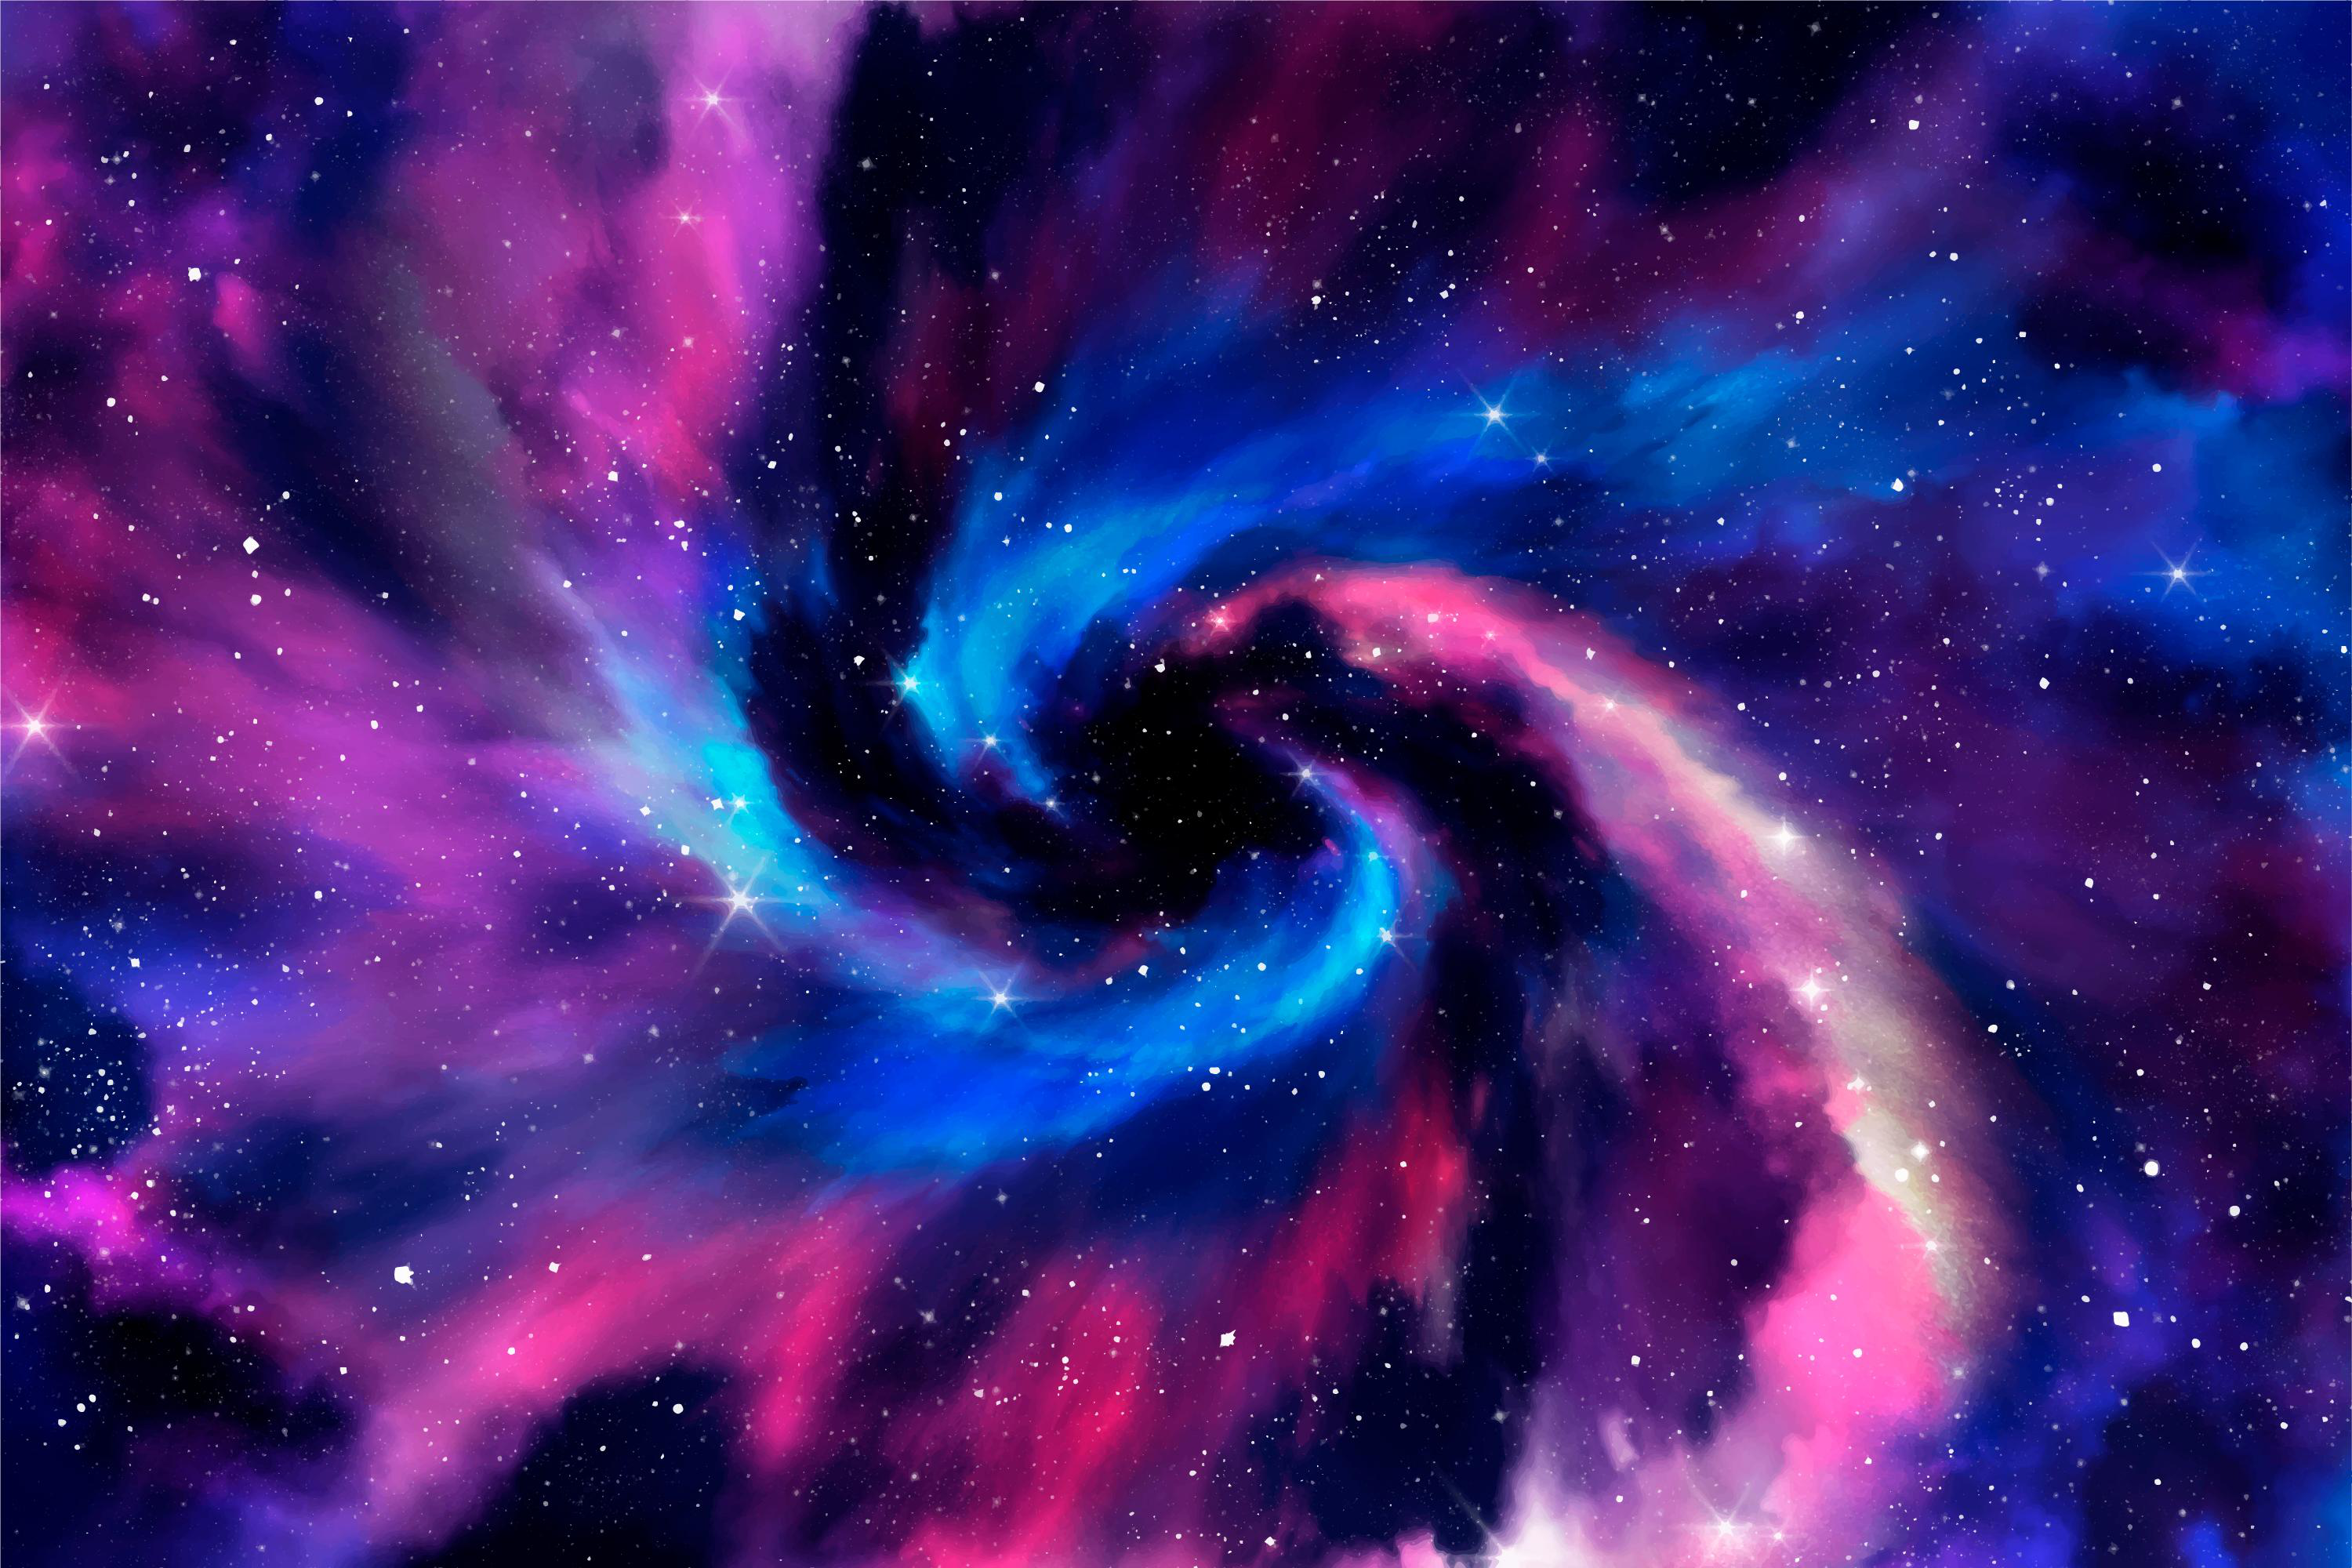
\includegraphics[width=4cm]{../Ch-acidbase/figure1}} node[rotate=90, font=\tiny] at ([yshift=.5cm,xshift=.1cm]a.south east) {\textsuperscript{\textcopyright} PngImg} ;
\end{tikzpicture}
\end{marginfigure}
   
  \import{files/}{ChapterIntro}
\begin{marginfigure}%LEARNING GOALS BOX
\begin{mytcbox}{GOALS}
\begin{enumerate}[label=\protect\circled{\color{white}\arabic*}]

\import{files/}{SectionGoal-Dissociation-of-acids-and-bases}
\import{files/}{SectionGoal-Dissociation-of-acids-and-base-Conjugate-organic-acids-and-bases}

\import{files/}{SectionGoal-Strength-of-acids-and-bases}
\import{files/}{SectionGoal-The-PH-scale}
\import{files/}{SectionGoal-Titrations}
\import{files/}{SectionGoal-Buffer-solutions}

\end{enumerate}
\end{mytcbox}
\vspace{1cm}
\begin{tcolorbox}[enhanced,colback=red!5!white,colframe=black!50!red,boxrule=1pt,
  arc=0pt,outer arc=0pt,drop heavy lifted shadow]
\faGears\ 
\docenvdef{Discussion:}   \import{files/}{ChapterDiscussion}
\end{tcolorbox}
\end{marginfigure}%LEARNING GOALS BOX
\section{\color{blue!30!black}{The nature of acids and Bases}}\import{files/}{SectionIntro-The-nature-of-acids-and-Bases}
 
\sloppy
\begin{description}
\item[\docfilehook{How to differentiate acids and bases based on their formula}{}] \import{files/}{SubSection-The-nature-of-acids-and-Bases-How-to-differentiate-acids-and-bases-based-on-their-formula}
  \import{problems/}{SampleProblem1}
 \import{files/}{SideFigure-Common-acids-and-bases}
\item[\docfilehook{ Acids and bases}{ }] \import{files/}{SubSection-The-nature-of-acids-and-Bases-Acids-and-bases}
\item[\docfilehook{Arrhenius acid-base model}{}] \import{files/}{SubSection-The-nature-of-acids-and-Bases-Arrhenius-acid-base-model}
\item[\docfilehook{Br\"{o}nsted-Lowry  acid-base model}{}]\import{files/}{SubSection-The-nature-of-acids-and-Bases-Bronsted-acids}
\item[\docfilehook{Lewis acid-base model}{}]\import{files/}{SubSection-The-nature-of-acids-and-Bases-Lewis-acid-base-model}
 \import{files/}{SideFigure-More-common-acids}
\import{files/}{SubSection-The-nature-of-acids-and-Bases-Acids-models-sumary}
 
 
  \import{files/}{Table-Acid-models}
  \import{problems/}{SampleProblem2}
\end{description}
\section{\color{blue!30!black}{Dissociation of acids and bases}}\import{files/}{SectionIntro-Dissociation-of-acids-and-bases}
\sloppy\begin{description}
\item[\docfilehook{ Conjugate acids and bases}{ }] \import{files/}{SubSection-Dissociation-of-acids-and-bases-Conjugate-acids-and-bases}
  \import{problems/}{SampleProblem3}
\item[\docfilehook{ Conjugate organic acids and bases}{ }] \import{files/}{SubSection-Dissociation-of-acids-and-base-Conjugate-organic-acids-and-bases}
  \import{problems/}{SampleProblem4}
\item[\docfilehook{ Writing down acid-base equilibria}{ }] \import{files/}{SubSection-Dissociation-of-acids-and-bases-Writing-down-acid-base-equilibria}
  \import{problems/}{SampleProblem5}
 \item[\docfilehook{ Dissociating organic acids and bases}{}] \import{files/}{SubSection-Dissociation-of-acids-and-bases-Dissociating-organic-acids-and-bases}
 
\end{description}
\section{\color{blue!30!black}{Strength of acids and bases}}\import{files/}{SectionIntro-Strength-of-acids-and-bases}
\sloppy\begin{description}
 
\item[\docfilehook{ Strength of acids and bases}{}] \import{files/}{SubSection-Strength-of-acids-and-bases-Strength-of-acids-and-bases-}
    \import{files/}{Table-Acidity-constants}
   \import{problems/}{SampleProblem6}
\item[\docfilehook{Including water in the dissociation}{}] \import{files/}{SubSection-Strength-of-acids-and-bases-Including-water-in-the-dissociation}
\item[\docfilehook{Acid-base properties of salts}{}] \import{files/}{SubSection-Strength-of-acids-and-bases-Acid-base-properties-of-salts}
  \import{problems/}{SampleProblem7}
 \import{files/}{SideFigure-PH-meter-and-indicators}
\end{description}
\section{\color{blue!30!black}{The PH scale}}\import{files/}{SectionIntro-The-PH-scale}
\sloppy
\begin{description}
\item[\docfilehook{ Protons and Hydroxyls}{}] \import{files/}{SubSection-The-PH-scale-Protons-and-Hydroxyls}
 
 
  \import{problems/}{SampleProblem8}
\item[\docfilehook{ The PH scale}{}] \import{files/}{SubSection-The-PH-scale-The-PH-scale}
  \import{files/}{Figure-PH-scale}
  \import{problems/}{SampleProblem9}
\item[\docfilehook{ PK of an acid or base}{}]\import{files/}{SubSection-The-PH-scale-PK-of-an-acid-or-base}
\item[\docfilehook{ From PH to proton concentration}{}] \import{files/}{SubSection-The-PH-scale-From-PH-to-proton-concentration}
  \import{problems/}{SampleProblem10}
  \import{files/}{Figure-PH-POH-formulas}
\item[\docfilehook{ PH of strong electrolyte solutions}{}] \import{files/}{SubSection-The-PH-scale-PH-of-strong-electrolyte-solutions}
  \import{problems/}{SampleProblem11}
\item[\docfilehook{ PH of solutions of weak acids and bases}{}] \import{files/}{SubSection-The-PH-scale-PH-of-solutions-of-weak-acids-and-bases}
  \import{problems/}{SampleProblem12}
  
  
\item[\docfilehook{ PH of salt solutions}{}] \import{files/}{SubSection-The-PH-scale-PH-of-salt-solutions}
  \import{problems/}{SampleProblem13}
\item[\docfilehook{ Percent dissociation of weak acids and bases}{}] \import{files/}{SubSection-The-PH-scale-Percent-dissociation-of-weak-acids-and-bases}
  \import{problems/}{SampleProblem14}
\end{description}
\section{\color{blue!30!black}{Buffer solutions}}\import{files/}{SectionIntro-Buffer-solutions}
\sloppy
\begin{description}
\item[\docfilehook{ Buffers}{}] \import{files/}{SubSection-Buffer-solutions-Buffers}
\item[\docfilehook{ PH of a Buffer solution}{}] \import{files/}{SubSection-Buffer-solutions-PH-of-a-Buffer-solution}
  \import{problems/}{SampleProblem15}
\item[\docfilehook{ PH of Buffer solution mixed with acids or bases}{}] \import{files/}{SubSection-Buffer-solutions-PH-of-Buffer-solution-mixed-with-acids-or-bases}
  \import{problems/}{SampleProblem16}
\end{description}
\section{\color{blue!30!black}{Titrations}}\import{files/}{SectionIntro-Titrations}
\sloppy
\begin{description}
\item[\docfilehook{ Neutralization Reactions}{}] \import{files/}{SubSection-Titrations-Neutralization-Reactions}
\item[\docfilehook{ Endpoint formula}{}] \import{files/}{SubSection-Titrations-Endpoint-formula}
  \import{files/}{Figure-Titration-curves}
  \import{problems/}{SampleProblem17}
\item[\docfilehook{ Titration curves}{}] \import{files/}{SubSection-Titrations-Titration-curves}
 
   
\item[\docfilehook{ Titration PH formulas}{}] 
\import{files/}{SubSection-Titrations-Titration-PH-formulas}
   \import{files/}{Table-Titration-formulas}
\item[\docfilehook{ $c_R$ and $c_F$}{}] 
\import{files/}{SubSection-Titrations-c_R-and-c_F}
   \import{problems/}{SampleProblem18}
  \import{problems/}{SampleProblem19}
\newpage
 
\end{description}
\section{\color{blue!30!black}{Blood as a buffer}}\import{files/}{SectionIntro-Blood-as-a-buffer}
 
\sloppy
\begin{description}
\item[\docfilehook{ Carbon dioxide is an acid}{}] \import{files/}{SubSection-Blood-as-a-buffer-Carbon-dioxide-is-an-acid}
\item[\docfilehook{ The dangerous change in blood PH}{}] 
\import{files/}{SubSection-Blood-as-a-buffer-The-dangerous-change-in-blood-PH}
  \import{files/}{Figure-Alkalosis-and-PH}
\item[\docfilehook{ Alkalosis and carbon dioxide}{}] 
\import{files/}{SubSection-Blood-as-a-buffer-Alkalosis-and-carbon-dioxide}
   \import{problems/}{SampleProblem20}
 \end{description}
 
 
 
%\begin{tikzpicture}
% \fill [blue,path fading=west] (0,0) rectangle (5cm,3mm);
% \fill [red,path fading=east, shift={(0em,0.7em)}] (0,0) rectangle (5cm,3mm);
%\fill [yellow,path fading=east, shift={(0em,-1.7em)}] (0,0) rectangle (2cm,3mm);
%\fill [green,path fading=west, shift={(0em,-0.7em)}] (3,0) rectangle (5cm,3mm);
%\end{tikzpicture}
\end{document}
